\documentclass{article}
\usepackage[a4paper, top=3cm, left=3cm, bottom=3cm, right=3cm]{geometry}
\usepackage[T1]{fontenc} 
\usepackage[utf8]{inputenc} 
\usepackage[italian]{babel} 
\usepackage{lipsum} 
\usepackage{url} 
\usepackage{lmodern}
\usepackage{graphicx}
\usepackage{psfrag}
\usepackage{amsfonts}
\usepackage{amsthm}
\usepackage{amsmath}
\usepackage{amssymb}
\usepackage{mathrsfs}
\usepackage{tikz-cd}
\usepackage{mathtools}
\usepackage{tikz} 
\usepackage{caption}
\captionsetup{labelformat=empty,textfont=sl}
\usetikzlibrary{decorations.markings}
\usepackage{enumitem}
\usepackage[hidelinks]{hyperref}
\usepackage[numbered,framed]{matlab-prettifier}

\lstset{
  style              = Matlab-editor,
  basicstyle         = \mlttfamily,
  escapechar         = ",
  mlshowsectionrules = true,
}

\title{\textbf{Laboratorio Sperimentale di Matematica Computazionale / / Mappa dei Colori}}
\author{Dario Rancati - 539365} 


\begin{document}

\maketitle

\noindent
La \texttt{function} estremamente semplice che realizza quanto richiesto dall'esercizio, cioè che prenda due interi $n$ ed $m$ in input e restituisca una griglia dei colori $n \times n$ con le sfumature di rosso e verde graduate da $1$ a $m$ (assumiamo dunque m<n). Per farla agiremo sulle prime due componenti dello standard rgb mettendo a zero la terza.

\begin{lstlisting}
function a = redgreen(n,m) 
    k=floor(n/m);
    for j = 1:n
        b(j)=floor(j/k)/m;
    end      
    a = zeros(n,n,3);
    a(:,:,1) = b'*ones(1,n);
    a(:,:,2) = ones(n,1)*b; 
    imshow(a);
end
\end{lstlisting}

\noindent
Con il comando \texttt{redgreen(256,200)} otteniamo la seguente immagine

\begin{figure}[h!]
\centering
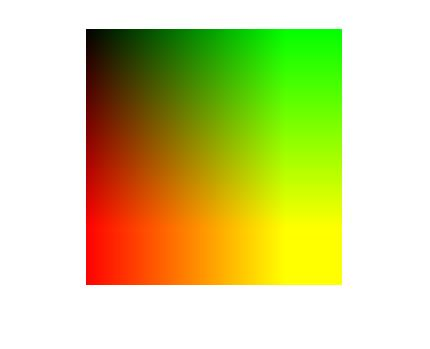
\includegraphics[width=\textwidth]{redgreen.jpg}
\end{figure}

\end{document}